\newpage
\section{数值积分与数值微分知识点概述}

\textcolor{blue}{1. 机械求积公式}

设给定一组节点 $ a \leqslant x_{0}<x_{1}<\cdots<x_{n} \leqslant b $, 且已知函数 $ f(x) $ 在这些节点上的值, 由插值或函数逼近近似代替得
$$
I(f)=\int_{a}^{b} f(x) d x \approx I_{n}(f)=\int_{a}^{b} \varphi(x) d x=\sum_{k=0}^{n} A_{k} f\left(x_{k}\right)
$$
这样构造出的求积公式称为机械求积公式, 其中, $ x_{k} $ 称为求积节点, $ A_{k} $ 称为求积系数.

\textcolor{blue}{2. 代数精确度}

若 $ I(f) $ 的求积公式
$$
I(f)=\int_{a}^{b} f(x) d x \approx I_{n}(f)=\sum_{k=0}^{n} A_{k} f\left(x_{k}\right)
$$
对所有的不高于 $ m $ 次多项式都准确成立, 但至少对 1 个 $ m+1 $ 次多项式是不准确成立的, 则称该求积公式具有 $ m $ 次代数精度 (或代数精确度). 实际应用过程中,只要利用多项式的基底来验证代数精度即可,比如求积公式 $ I_{n}(f) $ 对于 $ f(x)=x^{k}(k=0,1,2, \cdots, m) $ 均能准确成立, 但对 $ f(x)=x^{m+1} $不能准确成立.

\textcolor{blue}{3. 插值型求积}

设给定一组节点 $ a \leqslant x_{0}<x_{1}<\cdots<x_{n} \leqslant b $, 且已知函数 $ f(x) $ 在这些苦点上的值, 作 Lagrange 插值多项式
$$
L_{n}(x)=\sum_{k=0}^{n} l_{k}(x) f\left(x_{k}\right)
$$
其中, $ l_{k}(x)(k=0,1,2, \cdots, n) $ 为 $ n $ 次 Lagrange 插值基函数. 因此用 $ L_{n}(x) $ 近似代替被积函数 $ f(x) $ 可得
$$
I(f)=\int_{a}^{b} f(x) d x \approx I_{n}(f)=\sum_{k=0}^{n} A_{k} f\left(x_{k}\right)
$$
其中, $ A_{k}=\displaystyle\int_{a}^{b} l_{k}(x) d x $, 该机械求积公式的求积系数 $ A_{k} $ 由插值表达式得到, 则称该求积公式为插值型求积公式.

\textcolor{blue}{4. 求积公式余项}

积分真值 $ I(f)=\int_{a}^{b} f(x) d x $ 与求积公式给出的近似值之差, 称为求积公式的余项, 常用 $ R(f) $ 表示, 机械求积公式的余项
$$
R(f)=\int_{a}^{b}\left[f(x)-L_{n}(x)\right] d x=\int_{a}^{b} R_{n}(x) d x=\int_{a}^{b} \frac{f^{(n+1)}(\xi)}{(n+1)!} \omega_{n+1}(x) d x
$$
其中, $ \xi $ 依赖于 $ x $, 这里 $ \omega_{n+1}(x)=\left(x-x_{0}\right)\left(x-x_{1}\right) \cdots\left(x-x_{n}\right) $.通常地, 若被积函数 $ f(x) $ 是一个不高于 $ n $ 次的多项式, 由于 $ f^{(n+1)}(x)=0 $,其积分余项 $ R(f)=0 $, 因此, \textcolor{red}{$ n $ 阶插值多项式形式的数值积分公式至少有 $ n $ 阶代数精度.}

\textcolor{blue}{5. 牛顿-科茨 (Newton-Cotes) 公式}

求积系数 $ A_{k}=\int_{a}^{b} l_{k}(x) d x $ 与被积函数 $ f(x) $ 无关, 而与节点 $ x_{k} $ 及积分区间 $ [a, b] $ 有关, 在等距节点插值型求积公式的求积系数化简为
$$
A_{k}=\int_{a}^{b} l_{k}(x) d x=(b-a) C_{k}^{(n)}, \quad k=0,1, \cdots, n
$$
其中
$$
C_{k}^{(n)}=\frac{(-1)^{n-k}}{n k!(n-k)!} \int_{0}^{n} t(t-1) \cdots(t-k+1)(t-k-1) \cdots(t-n) d t
$$
显然 $ C_{k}^{(n)} $ 是一个仅与 $ n, k $ 有关, 与 $ f(x), a, b $ 都无关的常数, 称其为 Newton-Cotes 系数, 由此得到一个插值型求积公式
$$
I_{n}(f)=(b-a) \sum_{k=0}^{n} C_{k}^{(n)} f\left(x_{k}\right)
$$
这个积分公式称为 Newton-Cotes 求积公式.

一般地, 取 $ C_{0}^{(0)}=1 $, 利用函数的 Taylor 展开
$$
I(f)=\int_{a}^{b} f(x) d x=f\left(x_{0}\right)(b-a)+\int_{a}^{b}\left[f^{\prime}\left(x_{0}\right)\left(x-x_{0}\right)+\frac{f^{\prime \prime}\left(x_{0}\right)}{2!}\left(x-x_{0}\right)^{2}+\cdots\right] d x
$$
此时系数 $ C_{0}^{(0)}=1 $, 当 $ x_{0}=a, x_{0}=\frac{a+b}{2}, x_{0}=b $ 时, 分别称为
\begin{itemize}
    \item 左矩形公式: $ I(f) \approx f(a)(b-a) $.
    \item 中矩形公式: $ I(f) \approx f\left(\frac{a+b}{2}\right)(b-a) $.
    \item 右矩形公式: $ I(f) \approx f(b)(b-a) $.
\end{itemize}

\textcolor{blue}{6. 常用的 Newton-Cotes 求积公式}

\textbf{梯形公式 (两点公式)} 当 $ n=1 $ 时, 求积系数 $ C_{0}^{(1)}=C_{1}^{(1)}=\frac{1}{2} $, 因此
$$
T(f)=\frac{(b-a)}{2}(f(a)+f(b))
$$
梯形公式具有以下结论:
\begin{description}
    \item[(1)] 梯形公式的代数精度为 1 阶.
    \item[(2)] 梯形公式的余项为$\displaystyle R_{T}(f)=-\frac{(b-a)^{3}}{12} f^{\prime \prime}(\eta), \quad \eta \in(a, b)$
    \item[(3)] 几何意义是用梯形面积近似代替曲边梯形的面积.
\end{description}


\textbf{Simpson 公式 (三点公式或抛物公式)} 当 $ n=2 $ 时, 求积系数 $ C_{0}^{(2)}=\frac{1}{6} $, $ C_{1}^{(2)}=\frac{4}{6}, C_{2}^{(2)}=\frac{1}{6} $, 因此
$$
S(f)=\frac{b-a}{6}\left[f(a)+4 f\left(\frac{a+b}{2}\right)+f(b)\right]
$$
Simpson 公式具有以下结论:
\begin{description}
    \item[(1)] Simpson 公式的代数精度为 3 阶.
    \item[(2)]  Simpson 公式的余项为$\displaystyle R_{S}(f)=-\frac{(b-a)}{180} h^{4} f^{(4)}(\eta), \quad \eta \in(a, b)
$其中, $ h=\frac{b-a}{2} $.
    \item[(3)] 几何意义是 $ S(f) $ 是经过三点 $ (a, f(a)),\left(\frac{a+b}{2}\right. $, $ \left.f\left(\frac{a+b}{2}\right)\right),(b, f(b)) $ 的抛物线所围成的曲边梯形的面积.
\end{description}

\textbf{Cotes 公式 (五点公式)} 当 $ n=4 $ 时, Cotes 求积公式及其余项如下:
$$
\begin{aligned}
C(f)&=\frac{b-a}{90}\left[7 f\left(x_{0}\right)+32 f\left(x_{1}\right)+12 f\left(x_{2}\right)+32 f\left(x_{3}\right)+7 f\left(x_{4}\right)\right] \\
R_{C}(f)&=-\frac{2(b-a)}{945} h^{6} f^{(6)}(\eta), \quad \eta \in(a, b)
\end{aligned}
$$
其中, $ h=\frac{b-a}{4} $.
可以验证 Cotes 公式的代数精度为 5 阶, 且由梯形公式、Simpson 公式和 Cotes 公式的余项表达式我们能得到更一般的余项表述.

对于 Newton-Cotes 求积公式, 若 $ n $ 为偶数, 且 $ f(x) \in C^{n+2}[a, b] $, 则求积公式的误差余项为
$$
R(f)=\frac{h^{n+3} f^{(n+2)}(\xi)}{(n+2)!} \int_{0}^{n} t^{2}(t-1) \cdots(t-n) d t, \quad \xi \in(a, b)
$$
若 $ n $ 为奇数, 且 $ f(x) \in C^{n+1}[a, b] $, 则误差余项为
$$
R(f)=\frac{h^{n+2} f^{(n+1)}(\eta)}{(n+1)!} \int_{0}^{n} t(t-1) \cdots(t-n) d t, \quad \eta \in(a, b)
$$
因此, 当 $ n $ 为偶数时, 若被积函数 $ f(x) $ 是 $ n+1 $ 次多项式, 误差余项 $ R(f)=0 $,即求积公式对 $ n+1 $ 次多项式准确成立, 这表明此时该求积公式的代数精度可达到 $ n+1 $; 同理, 当 $ n $ 为奇数时, 该求积公式的代数精度可达到 $ n $.

\textcolor{blue}{7. 复化求积公式}

\textbf{复化梯形公式} \; 将求积区间 $ [a, b] $ 作 $ n $ 等分, 则步长 $ h=\frac{b-a}{n} $, 分点 $ x_{k}= $ $ a+k h, k=0,1,2, \cdots, n $, 对每一个小区间上的积分 $\displaystyle \int_{x_{k}}^{x_{k+1}} f(x) d x $ 应用梯形公式,得到复化梯形公式
$$
T_{n}(f)=\sum_{k=0}^{n-1} \frac{x_{k+1}-x_{k}}{2}\left[f\left(x_{k}\right)+f\left(x_{k+1}\right)\right]=\frac{h}{2} \sum_{k=0}^{n-1}\left[f\left(x_{k}\right)+f\left(x_{k+1}\right)\right]
$$
在复化梯形公式中, 每一个内节点 $ x_{1}, x_{2}, \cdots, x_{n-1} $, 既是前一个小区间的终点, 又是后一个小区间的起点, 因此又可以写为
$$
T_{n}(f)=\frac{h}{2}\left[f(a)+2 \sum_{k=1}^{n-1} f\left(x_{k}\right)+f(b)\right]
$$
复化梯形公式的余项为
$$
R_{T_{n}}(f)=I(f)-T_{n}(f)=\sum_{k=1}^{n}\left[-\frac{h^{3}}{12} f^{\prime \prime}\left(\eta_{k}\right)\right], \quad \eta_{k} \in\left(x_{k-1}, x_{k}\right)
$$
经过化简可得两种结果:
(1) 复化梯形公式的余项为
$$
R_{T_{n}}(f)=-\frac{(b-a)}{12} h^{2} f^{\prime \prime}(\eta), \quad \eta \in(a, b)
$$
(2) 复化梯形公式余项的近似表达式为
$$
R_{T_{n}}(f)=\sum_{k=1}^{n}\left[-\frac{h^{3}}{12} f^{\prime \prime}\left(\eta_{k}\right)\right] \approx-\frac{h^{2}}{12}\left[f^{\prime}(b)-f^{\prime}(a)\right]
$$

%利用余项复化梯形公式的端点修正公式
%$$
%\tilde{T}_{n}(f)=T_{n}(f)-\frac{h^{2}}{12}\left[f^{\prime}(b)-%f^{\prime}(a)\right]
%$$

\textbf{复化 Simpson 公式} \; 记 $ x_{k+\frac{1}{2}}=\frac{1}{2}\left(x_{k}+x_{k+1}\right) $, 对每一个小区间上的积分 $\displaystyle \int_{x_{k}}^{x_{k+1}} f(x) d x $ 应用 Simpson 公式, 可得复化 Simpson 公式
$$
S_{n}(f)=\sum_{k=0}^{n-1} \frac{h}{6}\left[f\left(x_{k}\right)+4 f\left(x_{k+\frac{1}{2}}\right)+f\left(x_{k+1}\right)\right]
$$
与复化梯形公式类似, 每个内节点 $ x_{1}, x_{2}, \cdots, x_{n} $ 需用两次, 因此有
$$
S_{n}(f)=\frac{h}{6}\left[f(a)+2 \sum_{k=1}^{n-1} f\left(x_{k}\right)+4 \sum_{k=0}^{n-1} f\left(x_{k+\frac{1}{2}}\right)+f(b)\right]
$$
复化 Simpson 的余项表达式
$$
R_{S_{n}}(f)=I(f)-S_{n}(f)=-\frac{h}{180}\left(\frac{h}{2}\right)^{4} \sum_{k=1}^{n} f^{(4)}\left(\eta_{k}\right), \quad \eta_{k} \in\left(x_{k-1}, x_{k}\right)
$$
经过化简可得两种结果:
(1) 复化 Simpson 公式的余项为
$$
R_{S_{n}}(f)=-\frac{b-a}{180}\left(\frac{h}{2}\right)^{4} f^{(4)}(\eta), \quad \eta \in(a, b)
$$
(2)复化 Simpson 公式余项的近似表达式为
$$
R_{S_{n}}(f) \approx-\frac{1}{180}\left(\frac{h}{2}\right)^{4}\left[f^{(3)}(b)-f^{(3)}(a)\right]
$$

\textbf{复化 Cotes 公式} \; 由复化求积思想, 记 $ x_{k+\frac{1}{4}}=x_{k}+\frac{1}{4} h, x_{k+\frac{1}{2}}=x_{k}+\frac{1}{2} h $, $ x_{k+\frac{3}{4}}=x_{k}+\frac{3}{4} h $ 对每一个小区上的积分 $\displaystyle \int_{x_{k}}^{x_{k+1}} f(x) d x $ 应用 Cotes 公式, 可得到复化 Cotes 公式
$$
C_{n}(f)=\sum_{k=0}^{n-1} \frac{h}{90}\left[7 f\left(x_{k}\right)+32 f\left(x_{k+\frac{1}{4}}\right)+12 f\left(x_{k+\frac{1}{2}}\right)+32 f\left(x_{k+\frac{3}{4}}\right)+7 f\left(x_{k+1}\right)\right]
$$
其误差余项为
$$
R_{C_{n}}(f)=I(f)-C_{n}(f)=-\frac{2(b-a)}{945}\left(\frac{h}{4}\right)^{6} f^{(6)}(\eta), \quad \eta \in(a, b)
$$

\textcolor{blue}{8. 复化求积公式的收敛阶}

对于复合求积公式 $\displaystyle \int_{a}^{b} f(x) d x \approx I_{n} $, 若当 $ h \rightarrow 0 $ 时, 有求积余项
$$
\frac{R_{n}(f)}{h^{p}}=\frac{\displaystyle\int_{a}^{b} f(x) d x-I_{n}}{h^{p}} \rightarrow c \quad(c \neq 0)
$$
则称复合求积公式 $ I_{n} $ 是 $ p $ 阶收敛的, 复化梯形公式、复化 Simpson 公式和复化 Cotes 公式的收敛阶分别具有 2 阶、 4 阶和 6 阶的收敛性.

\textcolor{blue}{9. 步长减半技术}

\textbf{复化梯形公式步长减半} \; 将积分区间 $ [a, b] $ 分成 $ n $ 个相等的子区间, 此时 $ h= $ $ \frac{b-a}{n} $, 由复化梯形公式的余项可得
$$
R_{T_{n}}(f)=I(f)-T_{n}(f) \approx-\frac{1}{12} h^{2}\left[f^{\prime}(b)-f^{\prime}(a)\right]
$$
将上述每个子区间二等分, 即将 $ [a, b] $ 分为 $ 2 n $ 个子区间, 则有
$$
E_{T_{2 n}}(f)=I(f)-T_{2 n}(f) \approx-\frac{1}{12}\left(\frac{h}{2}\right)^{2}\left[f^{\prime}(b)-f^{\prime}(a)\right]
$$
因此
$$
\frac{I(f)-T_{n}(f)}{I(f)-T_{2 n}(f)} \approx 4
$$
由此可得
$$
I(f) \approx T_{2 n}(f)+\frac{1}{3}\left[T_{2 n}(f)-T_{n}(f)\right]
\quad \text{或} \quad I(f) \approx \frac{4}{3} T_{2 n}(f)-\frac{1}{3} T_{n}(f)
$$

若 $ T_{2 n}(f) $ 作为积分真值 $ \int_{a}^{b} f(x) d x $ 的近似值, 其误差约为 $ \frac{1}{3}\left[T_{2 n}(f)-T_{n}(f)\right] $,即在区间逐次减半进行计算过程中, 可以用前后两次计算的结果 $ T_{2 n}(f) $ 和 $ T_{n}(f) $来估计误差与确定步长.

\textbf{复化 Simpson 公式和复化 Cotes 公式步长减半} \; 同样对于复化 Simpson 公式和复化 Cotes 公式, 由相应的余项公式也可以进行步长减半技术得到
$$
\frac{I(f)-S_{n}(f)}{I(f)-S_{2 n}(f)} \approx 16, \quad \frac{I(f)-C_{n}(f)}{I(f)-C_{2 n}(f)} \approx 64
$$
分别求解可得
$$
\begin{aligned}
I(f) &\approx S_{2 n}(f)+\frac{1}{15}\left[S_{2 n}(f)-S_{n}(f)\right] \\
I(f) &\approx C_{2 n}(f)+\frac{1}{63}\left[C_{2 n}(f)-C_{n}(f)\right]
\end{aligned}
$$

\textcolor{blue}{10. Gauss 型求积}

机械求积公式 $\displaystyle \int_{a}^{b} f(x) d x \approx \sum_{k=0}^{n} A_{k} f\left(x_{k}\right) $ 的代数精度不超过 $ 2 n+1 $ 阶.

若带权求积公式 $\displaystyle \int_{a}^{b} \rho(x) f(x) d x \approx \sum_{k=0}^{n} A_{k} f\left(x_{k}\right) $ 具有 $ 2 n+1 $ 次代数精度, 则称该公式为 Gauss 型求积公式, 求积公式的节点 $ x_{k}(k=0,1, \cdots, n) $ 称为 Gauss 点组. 其中, $ \rho(x) $ 为权函数,一般常用权函数 $ \rho(x)=1 $.

Gauss 型求积公式求解步骤为:
(1) 利用区间 $ [a, b] $ 上的 $ n+1 $ 次正交多项式确定 Gauss 点 $ x_{k}(k=0,1, \cdots, n) $;
(2) 利用 Gauss 点确定求积系数 $ A_{k}(k=0,1, \cdots, n) $.
若 $ n+1 $ 个节点 $ x_{0}, x_{1}, \cdots, x_{n} $ 是插值型求积公式
$$
\int_{a}^{b} \rho(x) f(x) d x \approx \sum_{k=0}^{n} A_{k} f\left(x_{k}\right)
$$
的 Gauss 点组的充分必要条件是 $ n+1 $ 次多项式 $ \omega_{n+1}(x)=\left(x-x_{0}\right)\left(x-x_{1}\right) \cdots(x $ 、 $ \left.x_{n}\right) $ 与任意次数不超过 $ n $ 的多项式 $ p(x) $ 正交, 即
$$
\int_{a}^{b} \rho(x) p(x) \omega_{n+1}(x) d x=0
$$

\textcolor{blue}{11. 利用插值多项式求导}

运用插值原理, 建立插值多项式 $ y=P_{n}(x) $ 作为它的近似, 取 $ P_{n}^{\prime}(x) $ 的值作为 $ f^{\prime}(x) $ 的近似值, 这样建立的数值公式 $ f^{\prime}(x) \approx P_{n}^{\prime}(x) $, 称为插值型的求导公式.
插值型的求导公式的余项为
$$
f^{\prime}(x)-P_{n}^{\prime}(x)=\frac{f^{(n+1)}(\xi)}{(n+1)!} \omega_{n+1}^{\prime}\left(x_{k}\right)
$$

两点公式
$$
\begin{aligned}
f^{\prime}\left(x_{0}\right) & =\frac{1}{h}\left[f\left(x_{1}\right)-f\left(x_{0}\right)\right]-\frac{h}{2} f^{\prime \prime}(\xi) \\
f^{\prime}\left(x_{1}\right) & =\frac{1}{h}\left[f\left(x_{1}\right)-f\left(x_{0}\right)\right]+\frac{h}{2} f^{\prime \prime}(\xi)
\end{aligned}
$$

三点公式
$$
\begin{aligned}
f^{\prime}\left(x_{0}\right)&=\frac{1}{2 h}\left[-3 f\left(x_{0}\right)+4 f\left(x_{1}\right)-f\left(x_{2}\right)\right]+\frac{h^{2}}{3} f^{\prime \prime \prime}\left(\xi_{0}\right) \\
f^{\prime}\left(x_{1}\right)&=\frac{1}{2 h}\left[-f\left(x_{0}\right)+f\left(x_{2}\right)\right]-\frac{h^{2}}{6} f^{\prime \prime \prime}\left(\xi_{1}\right) \\
f^{\prime}\left(x_{2}\right)&=\frac{1}{2 h}\left[f\left(x_{0}\right)-4 f\left(x_{1}\right)+3 f\left(x_{2}\right)\right]+\frac{h^{2}}{3} f^{\prime \prime \prime}\left(\xi_{2}\right)
\end{aligned}
$$

用插值多项式 $ P_{n}(x) $ 作为 $ f(x) $ 的近似函数, 还可以建立高阶数值微分公式:
$$
f^{(k)}(x) \approx P_{n}^{(k)}(x), \quad k=1,2, \cdots
$$


\newpage
\section{数值积分与数值微分理论推导}
\subsection{代数精度和节点数的关系}
\begin{tcolorbox}[enhanced,colback=2,colframe=1,breakable,coltitle=green!25!black,title=定理]
 对于给定的 $ n+1 $ 个 (相异) 节点 $ x_{k}, k=0,1, \cdots, n $, 总存在求积系数 $ A_{k} $, 使求积公式
$$
\int_{a}^{b} f(x) \mathrm{d} x \approx \sum_{k=0}^{n} A_{k} f\left(x_{k}\right)
$$
至少有 $ n $ 次代数精度.
\end{tcolorbox}
证: 令求积公式
$\displaystyle\int_{a}^{b} f(x) \mathrm{d} x \approx \sum_{k=0}^{n} A_{k} f\left(x_{k}\right)$ 对于 $ f(x)=1, x, x^{2}, \cdots, x^{n} $ 均准确成立, 可得
$$
\left\{\begin{array}{l}
A_{0}+A_{1}+\cdots+A_{n}=b-a \\
A_{0} x_{0}+A_{1} x_{1}+\cdots+A_{n} x_{n}=\frac{b^{2}-a^{2}}{2} \\
\vdots \\
A_{0} x_{0}^{n}+A_{1} x_{1}^{n}+\cdots+A_{n} x_{n}^{n}=\frac{b^{n+1}-a^{n+1}}{n+1}
\end{array}\right.
$$
只要证对 $ A_{k} $ 有唯一解即可.事实上, 上式是关于 $ A_{k} $ 的线性方程组, 其系数矩阵
$$
\left(\begin{array}{cccc}
1 & 1 & \cdots & 1 \\
x_{0} & x_{1} & \cdots & x_{n} \\
x_{0}^{2} & x_{1}^{2} & \cdots & x_{n}^{2} \\
\vdots & \vdots & & \vdots \\
x_{0}^{n} & x_{1}^{n} & \cdots & x_{n}^{n}
\end{array}\right)
$$
是范德蒙矩阵, 当 $ x_{k}(k=0,1, \cdots, n) $ 互异时非奇异, 故 $ A_{k} $ 有唯一解.因此, 对 $ f(x)=1, x, \cdots $, $ x^{n} $, 求积公式 $\displaystyle \int_{a}^{b} f(x) \mathrm{d} x \approx \sum_{k=0}^{n} A_{k} f\left(x_{k}\right) $ 准确成立, 故至少有 $ n $ 次代数精度.

\subsection{科茨系数之和为 1 }
\begin{center}
\begin{tabular}{c|ccccccc}
\hline$ n $ & $ C_{0}^{(n)} $ & $ C_{1}^{(n)} $ & $ C_{2}^{(n)} $ & $ C_{3}^{(n)} $ & $ C_{4}^{(n)} $ & $ C_{5}^{(n)} $ & $ C_{6}^{(n)} $ \\
\hline 1 & $ \frac{1}{2} $ & $ \frac{1}{2} $ & & & & \\
\hline 2 & $ \frac{1}{6} $ & $ \frac{4}{6} $ & $ \frac{1}{6} $ & & & \\
\hline 3 & $ \frac{1}{8} $ & $ \frac{3}{8} $ & $ \frac{3}{8} $ & $ \frac{1}{8} $ & & & \\
\hline 4 & $ \frac{7}{90} $ & $ \frac{16}{45} $ & $ \frac{2}{15} $ & $ \frac{16}{45} $ & $ \frac{7}{90} $ & \\
\hline 5 & $ \frac{19}{288} $ & $ \frac{25}{96} $ & $ \frac{25}{144} $ & $ \frac{25}{144} $ & $ \frac{25}{96} $ & $ \frac{19}{288} $ & \\
\hline 6 & $ \frac{41}{840} $ & $ \frac{9}{35} $ & $ \frac{9}{280} $ & $ \frac{34}{105} $ & $ \frac{9}{280} $ & $ \frac{9}{35} $ & $ \frac{41}{840} $ \\
\hline
\end{tabular}
\end{center}

科茨系数 $ C_{k} $ 与积分区间 $ [a, b] $ 及被积函数 $ f(x) $ 无关,仅与积分区间 $ [a, b] $ 的等分数 $ n $有关.此外, 从科茨系数表还可以看出: 科茨系数 $ C_{k} $ 之和为 1 , 即$\sum\limits_{k=0}^{n} C_{k}=1$

因为
$$
\begin{aligned}
\sum_{k=0}^{n} C_{k} & =\sum_{k=0}^{n} \frac{1}{b-a} \int_{a}^{b} l_{k}(x) \mathrm{d} x  =\frac{1}{b-a} \int_{a}^{b} \sum_{k=0}^{n} l_{k}(x) \mathrm{d} x=\frac{1}{b-a} \int_{a}^{b} 1 \mathrm{~d} x=1
\end{aligned}
$$






\newpage
\subsection{梯形公式、Simpson公式、科茨公式的截断误差}

(1)对于梯形公式$T(f)$,其具有\colorbox{yellow}{一次代数精度},有:
$$
R_{\mathrm{T}}(f)=I(f)-T(f)=\int_{a}^{b} \frac{f^{\prime \prime}(\xi)}{2}(x-a)(x-b) \mathrm{d} x,
$$
由于当 $ x \in(a, b) $ 时 $f^{\prime \prime}(\xi)$在区间$[a,b]$连续,而$(x-a)(x-b)$在该区间上不变号,即 $(x-a)(x-b)<0 $, 应用广义第一积分中值定理有
$$
\begin{aligned}
R_{\mathrm{T}}(f) & =\frac{f^{\prime \prime}(\eta)}{2} \int_{a}^{b}(x-a)(x-b) \mathrm{d} x  =\textcolor{blue}{\bm{-\frac{(b-a)^{3}}{12} f^{\prime \prime}(\eta)}}, \quad \eta \in(a, b) .
\end{aligned}
$$

(2)对于Simpson 公式 $ S(f) $, 其\colorbox{yellow}{代数精度为 3} , 因而对三次多项式是精确成立的. 对 $ f(x) $ 作满足下列插值条件的三次插值多项式 $ H_{3}(x) $ :
$$
H_{3}(a)=f(a), \quad H_{3}\left(\frac{a+b}{2}\right)  =f\left(\frac{a+b}{2}\right), \quad H_{3}(b)=f(b), \quad H_{3}^{\prime}\left(\frac{a+b}{2}\right)  =f^{\prime}\left(\frac{a+b}{2}\right) .
$$
满足上述插值条件的三次多项式 $ H_{3}(x) $ 是存在的,且有
$$
f(x)-H_{3}(x)=\frac{f^{(4)}(\xi)}{4!}(x-a)\left(x-\frac{a+b}{2}\right)^{2}(x-b),
$$
式中, $ \xi \in(\min \{x, a, b\}, \max \{x, a, b\}) $, 且 $ \xi $ 与 $ x $ 有关. 又
$$
\begin{aligned}
\int_{a}^{b} H_{3}(x) \mathrm{d} x  =S\left(H_{3}\right)&=\frac{b-a}{6}\left[H_{3}(a)+4 H_{3}\left(\frac{a+b}{2}\right)+H_{3}(b)\right] \\
& =\frac{b-a}{6}\left[f(a)+4 f\left(\frac{a+b}{2}\right)+f(b)\right]=S(f)
\end{aligned}
$$
因而
$$
\begin{aligned}
R_{\mathrm{S}}(f) & =I(f)-S(f)=\int_{a}^{b} f(x) \mathrm{d} x-\int_{a}^{b} H_{3}(x) \mathrm{d} x \\
& =\int_{a}^{b}\left[f(x)-H_{3}(x)\right] \mathrm{d} x \\
& =\int_{a}^{b} \frac{f^{(4)}(\xi)}{4!}(x-a)\left(x-\frac{a+b}{2}\right)^{2}(x-b) \mathrm{d} x \\
& =\frac{f^{(4)}(\eta)}{4!} \int_{a}^{b}(x-a)\left(x-\frac{a+b}{2}\right)^{2}(x-b) \mathrm{d} x \quad\text{\textcolor{red}{应用广义第一积分中值定理}}\\
& =\frac{f^{(4)}(\eta)}{4!} \int_{-1}^{1}(t+1) t^{2}(t-1)\left(\frac{b-a}{2}\right)^{5} \mathrm{~d} t \quad\text{\textcolor{red}{作变换}}\quad \textcolor{red}{x=\frac{a+b}{2}+\frac{b-a}{2}t}\\
& =\frac{f^{(4)}(\eta)}{4!} \cdot\left(\frac{b-a}{2}\right)^{5} \cdot 2 \int_{0}^{1} t^{2}\left(t^{2}-1\right) \mathrm{d} t \\
& =\textcolor{blue}{\bm{-\frac{b-a}{180}\left(\frac{b-a}{2}\right)^{4} f^{(4)}(\eta)}}, \quad \eta \in(a, b) .
\end{aligned}
$$

(3) 对于科茨公式 $ C(f) $, 它具有\colorbox{yellow}{ 5 次代数精度}, 其截断误差为
$$
R_{\mathrm{C}}(f)  =I(f)-C(f)  =\textcolor{blue}{\bm{-\frac{2(b-a)}{945}\left(\frac{b-a}{4}\right)^{6} f^{(6)}(\eta)}}, \quad \eta \in(a, b) .
$$
\newpage
\subsection{复化求积公式}
为简单起见, 将求积区间$[a,b]$作 $ n $ 等分, 并记
$$
h=\frac{b-a}{n}, \quad x_{i}=a+i h, \quad 0 \leqslant i \leqslant n,
$$
于是
$$
I(f)=\sum_{k=0}^{n-1} \int_{x_{k}}^{x_{k+1}} f(x) \mathrm{d} x
$$
并记
$$
I_{k}(f)=\int_{x_{k}}^{x_{k+1}} f(x) \mathrm{d} x .
$$

(1) 复化梯形公式

对每一个积分 $ I_{k}(f) $, 应用梯形公式, 得到复化梯形公式
$$
T_{n}(f)=\sum_{k=0}^{n-1} \frac{h}{2}\left[f\left(x_{k}\right)+f\left(x_{k+1}\right)\right]
$$
或者写成如下形式:
$$
T_{n}(f)=\frac{1}{2} h\left[f\left(a\right)+2 \sum_{k=1}^{n-1} f\left(x_{k}\right)+f\left(b\right)\right] .
$$

$$
\int_{x_{k}}^{x_{k+1}} f(x) \mathrm{d} x-\frac{h}{2}\left[f\left(x_{k}\right)+f\left(x_{k+1}\right)\right]=-\frac{h^{3}}{12} f^{\prime \prime}\left(\eta_{k}\right), \quad \eta_{k} \in\left(x_{k}, x_{k+1}\right),
$$

于是在 $ [a, b] $ 上复化梯形公式 $ T_{n}(f) $ 的截断误差为
$$
\begin{aligned}
I(f)-T_{n}(f) & =\sum_{k=0}^{n-1} \int_{x_{k}}^{x_{k+1}} f(x) \mathrm{d} x-\sum_{k=0}^{n-1} \frac{h}{2}\left[f\left(x_{k}\right)+f\left(x_{k+1}\right)\right] \\
& =\sum_{k=0}^{n-1}\left\{\int_{x_{k}}^{x_{k+1}} f(x) \mathrm{d} x-\frac{h}{2}\left[f\left(x_{k}\right)+f\left(x_{k+1}\right)\right]\right\} \\
& =\sum_{k=0}^{n-1}\left[-\frac{h^{3}}{12} f^{\prime \prime}\left(\eta_{k}\right)\right]=-\frac{h^{3}}{12} \sum_{k=0}^{n-1} f^{\prime \prime}\left(\eta_{k}\right) .
\end{aligned}
$$
设 $ f(x) \in C^{2}[a, b] $, 则由连续函数的介值定理知, 存在 $ \eta \in(a, b) $, 使得
$$
\frac{1}{n} \sum_{k=0}^{n-1} f^{\prime \prime}\left(\eta_{k}\right)=f^{\prime \prime}(\eta)
$$
于是
$$
I(f)-T_{n}(f)=-\frac{h^{3}}{12} n f^{\prime \prime}(\eta)=\textcolor{red}{\bm{-\frac{b-a}{12} f^{\prime \prime}(\eta) h^{2}}}, \quad \eta \in(a, b) .
$$
此外, 将上式两边同时除以 $ h^{2} $, 得
$$
\frac{I(f)-T_{n}(f)}{h^{2}}=-\frac{1}{12} h \sum_{k=0}^{n-1} f^{\prime \prime}\left(\eta_{k}\right) .
$$
注意到定积分的定义, 有
$$
\lim _{h \rightarrow 0}\left[h \sum_{k=0}^{n-1} f^{\prime \prime}\left(\eta_{k}\right)\right]=\int_{a}^{b} f^{\prime \prime}(x) \mathrm{d} x=f^{\prime}(b)-f^{\prime}(a)
$$
令 $ h \rightarrow 0 $, 并利用上式可得
$$
\lim _{h \rightarrow 0} \frac{I(f)-T_{n}(f)}{h^{2}}=-\frac{1}{12} \lim _{h \rightarrow 0}\left[h \sum_{k=0}^{n-1} f^{\prime \prime}\left(\eta_{k}\right)\right]=\frac{1}{12}\left[f^{\prime}(a)-f^{\prime}(b)\right] .
$$
因而当 $ h $ 适当小时, 有
$$
\frac{I(f)-T_{n}(f)}{h^{2}} \approx \frac{1}{12}\left[f^{\prime}(a)-f^{\prime}(b)\right]
$$
或
$$
I(f)-T_{n}(f) \approx \frac{1}{12}\left[f^{\prime}(a)-f^{\prime}(b)\right] h^{2} .
$$

(2)复化Simpson公式

记 $ x_{k+\frac{1}{2}}=\frac{1}{2}\left(x_{k}+x_{k+1}\right) $. 对每一个积分 $ I_{k}(f) $ 应用Simpson公式, 得到复化Simpson公式

$$
S_{n}(f)=\sum_{k=0}^{n-1} \frac{h}{6}\left[f\left(x_{k}\right)+4 f\left(x_{k+\frac{1}{2}}\right)+f\left(x_{k+1}\right)\right]
$$
或
$$
S_{n}(f)=\frac{h}{6}\left[f\left(a\right)+2 \sum_{k=1}^{n-1} f\left(x_{k}\right)+f\left(b\right)+4 \sum_{k=0}^{n-1} f\left(x_{k+\frac{1}{2}}\right)\right] .
$$
则
$$
 \int_{x_{k}}^{x_{k+1}} f(x) \mathrm{d} x-\frac{h}{6}\left[f\left(x_{k}\right)+4 f\left(x_{k+\frac{1}{2}}\right)+f\left(x_{k+1}\right)\right] =  -\frac{h}{180}\left(\frac{h}{2}\right)^{4} f^{(4)}\left(\eta_{k}\right), \quad \eta_{k} \in\left(x_{k}, x_{k+1}\right),
$$
于是在 $ [a, b] $ 上复化Simpson公式的截断误差为
$$
\begin{aligned}
I(f)-S_{n}(f) & =\sum_{k=0}^{n-1}\left\{\int_{x_{k}}^{x_{k+1}} f(x) \mathrm{d} x-\frac{h}{6}\left[f\left(x_{k}\right)+4 f\left(x_{k+\frac{1}{2}}\right)+f\left(x_{k+1}\right)\right]\right\} \\
& =\sum_{k=0}^{n-1}\left[-\frac{h}{180}\left(\frac{h}{2}\right)^{4} f^{(4)}\left(\eta_{k}\right)\right] \\
& =-\frac{h}{180}\left(\frac{h}{2}\right)^{4} \sum_{k=0}^{n-1} f^{(4)}\left(\eta_{k}\right) .
\end{aligned}
$$
设 $ f(x) \in C^{4}[a, b] $, 则由连续函数的介值定理知, 存在 $ \eta \in(a, b) $, 使得
$$
\frac{1}{n} \sum_{k=0}^{n-1} f^{(4)}\left(\eta_{k}\right)=f^{(4)}(\eta)
$$
因此有
$$
I(f)-S_{n}(f)  =-\frac{h}{180}\left(\frac{h}{2}\right)^{4} n f^{(4)}(\eta)  =\textcolor{red}{\bm{-\frac{b-a}{180} f^{(4)}(\eta)\left(\frac{h}{2}\right)^{4}}}, \quad \eta \in(a, b) .
$$
此外, 将上式的两边同时除以 $ \left(\frac{h}{2}\right)^{4} $, 得
$$
\frac{I(f)-S_{n}(f)}{\left(\frac{h}{2}\right)^{4}}=-\frac{1}{180} h \sum_{k=0}^{n-1} f^{(4)}\left(\eta_{k}\right) .
$$
注意到定积分的定义, 有
$$
\lim _{h \rightarrow 0}\left[h \sum_{k=0}^{n-1} f^{(4)}\left(\eta_{k}\right)\right]=\int_{a}^{b} f^{(4)}(x) \mathrm{d} x=f^{(3)}(b)-f^{(3)}(a),
$$
令 $ h \rightarrow 0 $, 并利用上式可得
$$
\lim _{h \rightarrow 0} \frac{I(f)-S_{n}(f)}{\left(\frac{h}{2}\right)^{4}}=-\frac{1}{180} \lim _{h \rightarrow 0}\left[h \sum_{k=0}^{n-1} f^{(4)}\left(\eta_{k}\right)\right]=\frac{1}{180}\left[f^{(3)}(a)-f^{(3)}(b)\right] .
$$
因而当 $ h $ 适当小时, 有
$$
\frac{I(f)-S_{n}(f)}{\left(\frac{h}{2}\right)^{4}} \approx \frac{1}{180}\left[f^{(3)}(a)-f^{(3)}(b)\right]
$$
或
$$
I(f)-S_{n}(f) \approx \frac{1}{180}\left[f^{(3)}(a)-f^{(3)}(b)\right]\left(\frac{h}{2}\right)^{4} .
$$

(3) 复化科茨公式

记 $x_{k+\frac{1}{4}}=x_{k}+\frac{1}{4} h, x_{k+\frac{1}{2}}=x_{k}+\frac{1}{2} h, x_{k+\frac{3}{4}}=x_{k}+\frac{3}{4} h$ , 对每一个积分 $I_{k}(f)$  应用科茨公式, 得到复化科茨公式
$$
C_{n}(f)=\sum_{k=0}^{n-1} \frac{h}{90}\left[7 f\left(x_{k}\right)+32 f\left(x_{k+\frac{1}{4}}\right)+12 f\left(x_{k+\frac{1}{2}}\right)+32 f\left(x_{k+\frac{3}{4}}\right)+7 f\left(x_{k+1}\right)\right] .
$$
类似对复化梯形公式和复化Simpson公式的分析, 可得复化科茨公式的截断误差为
$$
I(f)-C_{n}(f)=\textcolor{red}{\bm{-\frac{2(b-a)}{945} f^{(6)}(\eta)\left(\frac{h}{4}\right)^{6}}}, \quad \eta \in(a, b),
$$
且当 $ h $ 适当小时, 有
$$
I(f)-C_{n}(f) \approx \frac{2}{945}\left[f^{(5)}(a)-f^{(5)}(b)\right]\left(\frac{h}{4}\right)^{6} .
$$

\subsection{Romberg求积法}
根据前面我们知道:
$$\begin{aligned}
    I(f)-T_{n}(f) &\approx \frac{1}{12}\left[f^{\prime}(a)-f^{\prime}(b)\right] h^{2} \\
    I(f)-T_{2 n}(f) &\approx \frac{1}{12}\left[f^{\prime}(a)-f^{\prime}(b)\right]\left(\frac{h}{2}\right)^{2} .
\end{aligned}
$$
将商面两式结合起来可以写成如下形式:
$$
I(f)-T_{2 n}(f) \approx \frac{1}{4}\left[I(f)-T_{n}(f)\right],
$$
上式两边乘以 $ \frac{4}{3} $, 再移项得
$$
I(f)-T_{2 n}(f) \approx \frac{1}{3}\left[T_{2 n}(f)-T_{n}(f)\right] .
$$
于是复化梯形公式的误差估计式为
$$
I(f)-T_{2 n}(f) \approx \frac{1}{3}\left[T_{2 n}(f)-T_{N}(f)\right],
$$
我们用此误差估计式对 $ T_{2 n}(f) $ 进行修正, 有
$$
\begin{aligned}
\widetilde{T}_{n}(f) & =T_{2 n}(f)+\frac{1}{3}\left[T_{2 n}(f)-T_{n}(f)\right] \\
& =\frac{4}{3} T_{2 n}(f)-\frac{1}{3} T_{n}(f) .
\end{aligned}
$$
以上 $ T_{2 n}(f) $ 和 $ T_{n}(f) $ 均是 $ I(f) $ 的 2 阶近似, 将它们作线性组合后其精度是否发生大的变化了呢? 由复化梯形公式
$$
T_{n}(f)=\sum_{k=0}^{n-1} \frac{h}{2}\left[f\left(x_{k}\right)+f\left(x_{k+1}\right)\right]
$$
并记
$$
x_{k+\frac{1}{2}}=\frac{1}{2}\left(x_{k}+x_{k+1}\right), \quad k=0,1, \cdots, n-1,
$$
则
$$
\begin{aligned}
T_{2 n}(f) & =\sum_{k=0}^{n-1}\left\{\frac{1}{2} \cdot \frac{h}{2}\left[f\left(x_{k}\right)+f\left(x_{k+\frac{1}{2}}\right)\right]+\frac{1}{2} \cdot \frac{h}{2}\left[f\left(x_{k+\frac{1}{2}}\right)+f\left(x_{k+1}\right)\right]\right\} \\
& =\frac{1}{2} \sum_{k=0}^{n-1} \frac{h}{2}\left[f\left(x_{k}\right)+f\left(x_{k+1}\right)\right]+\frac{1}{2} h \sum_{k=0}^{n-1} f\left(x_{k+\frac{1}{2}}\right) \\
& =\frac{1}{2}\left[T_{n}(f)+h \sum_{k=0}^{n-1} f\left(x_{k+\frac{1}{2}}\right)\right] .
\end{aligned}
$$
将二者代入$\widetilde{T}_{n}(f)$中,于是有
$$
\begin{aligned}
\widetilde{T}_{n}(f)= & \frac{4}{3} \sum_{k=0}^{n-1}\left\{\frac{h}{4}\left[f\left(x_{k}\right)+f\left(x_{k+\frac{1}{2}}\right)\right]+\frac{h}{4}\left[f\left(x_{k+\frac{1}{2}}\right)+f\left(x_{k+1}\right)\right]\right\}  -\frac{1}{3} \sum_{k=0}^{n-1} \frac{h}{2}\left[f\left(x_{k}\right)+f\left(x_{k+1}\right)\right] \\
= & \sum_{k=0}^{n-1}\left\{\frac{h}{3}\left[f\left(x_{k}\right)+2 f\left(x_{k+\frac{1}{2}}\right)+f\left(x_{k+1}\right)\right]-\frac{h}{6}\left[f\left(x_{k}\right)+f\left(x_{k+1}\right)\right]\right\} \\
= & \sum_{k=0}^{n-1} \frac{h}{6}\left[f\left(x_{k}\right)+4 f\left(x_{k+\frac{1}{2}}\right)+f\left(x_{k+1}\right)\right] \\
= & S_{n}(f),
\end{aligned}
$$
即
$$
\textcolor{red}{S_{n}(f)=\frac{4}{3} T_{2 n}(f)-\frac{1}{3} T_{n}(f) .}
$$

显然, 用复化梯形公式算出的二分前后两个积分值 $ T_{n}(f) $ 和 $ T_{2 n}(f) $ 按线性组合所得, 实际上就是用复化 Simpson 公式求得的近似值 $ S_{n}(f) $.用同样的思想来研究复化 Simpson 公式的加速问题. 由前面知复化 Simpson 公式的误差估计式为
$$
I(f)-S_{2 n}(f) \approx \frac{1}{15}\left[S_{2 n}(f)-S_{n}(f)\right]
$$
用这一估计式对 $ S_{2 n}(f) $ 进行修正, 得到
$$
\begin{aligned}
\tilde{S}_{n}(f) & =S_{2 n}(f)+\frac{1}{15}\left[S_{2 n}(f)-S_{n}(f)\right]  =\frac{16}{15} S_{2 n}(f)-\frac{1}{15} S_{n}(f) .
\end{aligned}
$$
直接验证可知上式右端的值就是复化 $ \operatorname{Cotes} $ 公式所得积分值 $ C_{n}(f) $, 即
$$
C_{n}(f)=\frac{16}{15} S_{2 n}(f)-\frac{1}{15} S_{n}(f) .
$$

重复上述方法,复化 Cotes 公式的误差估计式为
$$
I(f)-C_{2 n}(f) \approx \frac{1}{63}\left[C_{2 n}(f)-C_{n}(f)\right],
$$
用这一误差估计式对 $ C_{2 n}(f) $ 进行修正, 得到计算积分 $ I(f) $ 的一个新的求解公式
$$
\begin{aligned}
R_{n}(f) & =C_{2 n}(f)+\frac{1}{63}\left[C_{2 n}(f)-C_{n}(f)\right] =\textcolor{red}{\frac{64}{63} C_{2 n}(f)-\frac{1}{63} C_{n}(f)}
\end{aligned}
$$
该式为计算$I(f)$ 的Romberg 公式,其具有\colorbox{yellow}{七次代数精度},截断误差为$O(h^8)$.
\subsection{Gauss 求积公式}

\begin{tcolorbox}[enhanced,colback=yellow!5!white,colframe=yellow!50!black,colbacktitle=yellow!80!black,title=定义]
    设计算积分 $ I(f)=\int_{a}^{b} f(x) \mathrm{d} x $ 的求积公式为
$$
I_{n}(f)=\sum_{k=0}^{n} A_{k} f\left(x_{k}\right),
$$

如果其代数精度为 $ 2 n+1 $, 则称该求积公式为 Gauss-Legendre 公式(简称Gauss公式), 称相应的求积节点为 Gauss 点.
\end{tcolorbox}

由代数精度的定义知, $\displaystyle I_{n}(f)=\sum_{k=0}^{n} A_{k} f\left(x_{k}\right)$ 为 Gauss 公式的充要条件是求积节点 $ \left\{x_{k}\right\rangle_{k-0}^{n} $和求积系数 $ \left\{A_{k}\right\rangle_{k=0}^{n} $ 满足下列方程组:
$$
\left\{\begin{array}{l}\displaystyle
\displaystyle\sum_{k=0}^{n} A_{k}=\int_{a}^{b} 1 \mathrm{~d} x, \\
\displaystyle\sum_{k=0}^{n} x_{k} A_{k}=\int_{a}^{b} x \mathrm{~d} x, \\
\displaystyle\sum_{k=0}^{n} x_{k}^{2} A_{k}=\int_{a}^{b} x^{2} \mathrm{~d} x, \\
\vdots \\
\displaystyle\sum_{k=0}^{n} x_{k}^{2 n+1} A_{k}=\int_{a}^{b} x^{2 n+1} \mathrm{~d} x .
\end{array}\right.
$$


\begin{tcolorbox}[enhanced,colback=2,colframe=1,breakable,coltitle=green!25!black,title=定理]
若 $ f(x) \in C^{2 n+2}[a, b] $, 则其 Gauss 公式
$\displaystyle\int_{a}^{b} f(x) \mathrm{d} x \approx \sum_{k=0}^{n} A_{k} f\left(x_{k}\right)$的截断误差为
$$
\begin{aligned}
R(f) & =\int_{a}^{b} f(x) \mathrm{d} x-\sum_{k=0}^{n} A_{k} f\left(x_{k}\right) =\frac{f^{(2 n+2)}(\xi)}{(2 n+2)!} \int_{a}^{b} W_{n+1}^{2}(x) \mathrm{d} x,
\end{aligned}
$$
其中 $ W_{n+1}(x)=\left(x-x_{0}\right)\left(x-x_{1}\right) \cdots\left(x-x_{n}\right), \xi \in(a, b) $.
 \end{tcolorbox}

推论:设计算 $ I(f)=\displaystyle\int_{a}^{b} f(x) \mathrm{d} x $ 的求积公式为$I_{n}(f)=\displaystyle\sum_{k=0}^{n} A_{k} f\left(x_{k}\right),$
则其代数精度最多为 $ 2 n+1 $.

\subsection{数值微分}

根据函数在一些离散点上的函数值推算它在其占外导数的近似值的方法称为 数值微分. 取间单的数值微分公式是用向前差商近似代替导数, 即

$$f^{{\prime}}\left( x_{0} \right) {\approx} \frac{f\left( x_{0} + h \right) {-} f\left( x_{0} \right)}{h}.$$
类似地,也可用向后差商近似代替导数,即
$$f^{{\prime}}\left( x_{0} \right) {\approx} \frac{f\left( x_{0} \right) {-} f\left( x_{0} {-} h \right)}{h},$$
或用中心差商近似代替导数,即
$$f^{{\prime}}\left( x_{0} \right) {\approx} \frac{f\left( x_{0} + h \right) {-} f\left( x_{0} {-} h \right)}{2h}.$$

\begin{window}[0,r,{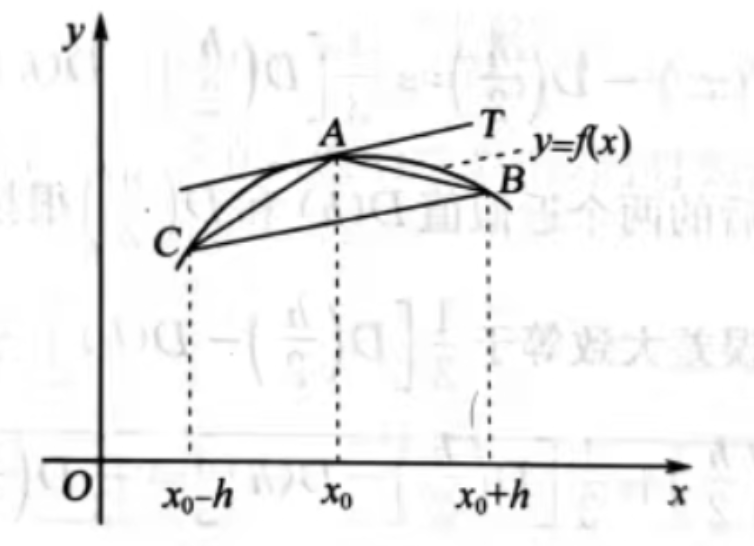
\includegraphics[width=6cm]{0.png}},{}]
 在如图所示的几何图形上,这三种差商分别表示弦 $AB,AC$ 和 $BC$ 的斜率 将这三条弦同过 $A$ 点的切线 $AT$ 相比较,一般地说,弦 $BC$ 的斜率更接近于切线 $AT$  的斜率 $f\left( x_{0} \right)$ ,因此就精度而言,第三个式子更为可取. 
 我们称
$D(h) = \dfrac{f\left( x_{0} + h \right) {-} f\left( x_{0} {-} h \right)}{2h}$为求 $f^{{\prime}}\left( x_{0} \right)$ 的中点公式.
现在来考察用中点公式 代替 $f^{{\prime}}\left( x_{0} \right)$ 所产生的截断误差 $f^{{\prime}}\left( x_{0} \right) {-} D(h)$ . 由泰 勒展开式有
\end{window}



$$\begin{aligned}
    f^{{\prime}}\left( x_{0} \right) {-} D(h) &= f^{{\prime}}\left( x_{0} \right) {-} \frac{1}{2h}\left\lbrack f\left( x_{0} + h \right) {-} f\left( x_{0} {-} h \right) \right\rbrack\\
    &= f^{{\prime}}\left( x_{0} \right) {-} \frac{1}{2h}\left\{\lbrack f\left( x_{0} \right) + hf^{{\prime}}\left( x_{0} \right) + \frac{1}{2}h^{2}f^{{\prime}{\prime}}\left( x_{0} \right)  +\frac{1}{6}h^{3}f^{{\prime}{\prime}{\prime}}\left( x_{0} + {\theta}_{1}h \right) \right\rbrack \\&{-} \left\lbrack f\left( x_{0} \right) {-} hf^{{\prime}}\left( x_{0} \right) \right.\left. \left. +\frac{1}{2}h^{2}f^{{\prime}{\prime}}\left( x_{0} \right) {-} \frac{1}{6}h^{3}f^{{\prime}{\prime}{\prime}}\left( x_{0} {-} {\theta}_{2}h \right) \right\rbrack \right\}\\
    &=-\frac{1}{12} h^{2}\left[f^{\prime \prime}\left(x_{0}+\theta_{1} h\right)+f^{\prime \prime}\left(x_{0}-\theta_{2} h\right)\right] \\
&=-\frac{1}{6} h^{2} f^{\prime \prime}\left(x_{0}+\theta h\right),
\end{aligned}$$
其中, $ \theta_{1}, \theta_{2} \in(0,1), \theta \in(-1,1) $.
从截断误差的角度来看,步长 $ h $ 越小,计算结果越精确. 但从舍入误差的角度看, 如果 $ h $ 越小, 则 $ f\left(x_{0}+h\right) $ 与 $ f\left(x_{0}-h\right) $ 越接近, 直接相减会造成有效数字的严重损失, 因此步长 $ h $ 不宜太小. %那怎样选取合适的步长呢? 可采用二分步长及事后误差估计法.

由以上讨论可知,对于中点公式,若以缩小步长 $h$ 来提高精度,那么只能适合于用解析式表示的函数,对于列表函数的求导,若要提高精度,还需另想别的方法.

对于列表函数 $y=f(x)$:
\begin{center}
\begin{tabular}{c|cccc}
$ x $ & $ x_{0} $ & $ x_{1} $ & $ \cdots $ & $ x_{n} $ \\
\hline$ y $ & $ y_{0} $ & $ y_{1} $ & $ \cdots $ & $ y_{n} $
\end{tabular}
\end{center}
应用插值原理, 可以建立插值多项式 $ p_{n}(x) $ 作为 $ f(x) $ 的近似. 由于多项式的求导比较容易, 因此可以取 $ p_{n}^{\prime}(x) $ 的值作为 $ f^{\prime}(x) $ 的近似值, 这样建立的数值公式
$$
f^{\prime}(x) \approx p_{n}^{\prime}(x)
$$
统称为\textbf{插值型求导公式}.

插值型求导公式 $ p_{n}^{\prime}(x) $ 的截断误差由插值余项
$$
f(x)-p_{n}(x)=\frac{f^{(n+1)}(\xi)}{(n+1)!} W_{n+1}(x)
$$
求导数得到. 因为
$$
\begin{array}{c}
\xi=\xi(x) \in\left(\min \left\{x, x_{0}, \cdots, x_{n}\right\}, \max \left\{x, x_{0}, \cdots, x_{n}\right\}\right), \\
W_{n+1}(x)=\left(x-x_{0}\right)\left(x-x_{1}\right) \cdots\left(x-x_{n}\right),
\end{array}
$$
于是 $ p_{n}^{\prime}(x) $ 的截断误差为
$$
f^{\prime}(x)-p_{n}^{\prime}(x)=\frac{f^{(n+1)}(\xi)}{(n+1)!} W_{n+1}^{\prime}(x)+\frac{W_{n+1}(x)}{(n+1)!} \frac{\mathrm{d}}{\mathrm{d} x} f^{(n+1)}(\xi) .
$$
上面的公式中, $ \xi $ 是 $ x $ 的未知函数, 很难对 $ \frac{\mathrm{d}}{\mathrm{d} x} f^{(n+1)}(\xi) $ 作进一步的估计. 若限定在某个节点 $ x_{k} $ 上求导数, 并注意到 $ W_{n+1}\left(x_{k}\right)=0 $, 此时 $ p^{\prime}{ }_{n}\left(x_{k}\right) $ 的截断误差表达式变得很简单, 即有
$$
f^{\prime}\left(x_{k}\right)-p_{n}^{\prime}\left(x_{k}\right)=\frac{f^{(n+1)}(\xi)}{(n+1)!} W_{n+1}^{\prime}\left(x_{k}\right)=\frac{f^{(n+1)}(\xi)}{(n+1)!} \prod_{\substack{j=0 \\ j \neq k}}^{n}\left(x_{k}-x_{j}\right) .
$$

由于以上的原因,下面仅考虑节点处的导数值.

(1) 两点公式

已知列表函数 $ y=f(x): $
\begin{tabular}{c|cc}
$ x $ & $ x_{0} $ & $ x_{1} $ \\
\hline$ y $ & $ f\left(x_{0}\right) $ & $ f\left(x_{1}\right) $
\end{tabular}
作一次插值多项式
$$
p_{1}(x)=\frac{x-x_{1}}{x_{0}-x_{1}} f\left(x_{0}\right)+\frac{x-x_{0}}{x_{1}-x_{0}} f\left(x_{1}\right) .
$$
对上式两端求导, 并记 $ h=x_{1}-x_{0} $, 则有
$$
p_{1}^{\prime}(x)=\frac{1}{h}\left[-f\left(x_{0}\right)+f\left(x_{1}\right)\right]
$$
于是有下列求导公式:
$$
p_{1}^{\prime}\left(x_{0}\right)=\frac{1}{h}\left[f\left(x_{1}\right)-f\left(x_{0}\right)\right], \quad p_{1}^{\prime}\left(x_{1}\right)=\frac{1}{h}\left[f\left(x_{1}\right)-f\left(x_{0}\right)\right],
$$

这与已介绍的向前差商与向后差商公式 是一致的. 而 $ p_{1}^{\prime}\left(x_{0}\right)=p_{1}^{\prime}\left(x_{1}\right) $ 是不奇怪的,因为 $ A, B $ 两点处的导数都以直线 $ A B $ 的斜率为近似值. 但它们的截断误差应该是不同的. 事实上, 有
$$
\begin{aligned}
f^{\prime}\left(x_{0}\right)-p_{1}^{\prime}\left(x_{0}\right)&=\frac{f^{\prime \prime}\left(\xi_{0}\right)}{2!} W_{2}^{\prime}\left(x_{0}\right)=\frac{f^{\prime \prime}\left(\xi_{0}\right)}{2}\left(x_{0}-x_{1}\right)=-\frac{h}{2} f^{\prime \prime}\left(\xi_{0}\right), \\
f^{\prime}\left(x_{1}\right)-p_{1}^{\prime}\left(x_{1}\right)&=\frac{f^{\prime \prime}\left(\xi_{1}\right)}{2!} W_{2}^{\prime}\left(x_{1}\right)=\frac{f^{\prime}\left(\xi_{1}\right)}{2}\left(x_{1}-x_{0}\right)=\frac{h}{2} f^{\prime \prime}\left(\xi_{1}\right),
\end{aligned}
$$
因此带余项的两点公式为
$$
\begin{aligned}
f^{\prime}\left(x_{0}\right)&=\frac{1}{h}\left[f\left(x_{1}\right)-f\left(x_{0}\right)\right]-\frac{h}{2} f^{\prime \prime}\left(\xi_{0}\right), \quad x_{0}<\xi_{0}<x_{1}, \\
f^{\prime}\left(x_{1}\right)&=\frac{1}{h}\left[f\left(x_{1}\right)-f\left(x_{0}\right)\right]+\frac{h}{2} f^{\prime \prime}\left(\xi_{1}\right), \quad x_{0}<\xi_{1}<x_{1} . \\
\end{aligned}
$$

(2) 三点公式

已知列表函数 $ y=f(x) $ :
\begin{tabular}{c|ccc}
$ x $ & $ x_{0} $ & $ x_{1} $ & $ x_{2} $ \\
\hline$ y $ & $ f\left(x_{0}\right) $ & $ f\left(x_{1}\right) $ & $ f\left(x_{2}\right) $
\end{tabular}
作 2 次插值多项式
$$
\begin{aligned}
p_{2}(x)= & \frac{\left(x-x_{1}\right)\left(x-x_{2}\right)}{\left(x_{0}-x_{1}\right)\left(x_{0}-x_{2}\right)} f\left(x_{0}\right)+\frac{\left(x-x_{0}\right)\left(x-x_{2}\right)}{\left(x_{1}-x_{0}\right)\left(x_{1}-x_{2}\right)} f\left(x_{1}\right)  +\frac{\left(x-x_{0}\right)\left(x-x_{1}\right)}{\left(x_{2}-x_{0}\right)\left(x_{2}-x_{1}\right)} f\left(x_{2}\right) .
\end{aligned}
$$
对 $ p_{2}(x) $ 求导, 得
$$
\begin{aligned}
p_{2}^{\prime}(x)= & \frac{2 x-x_{1}-x_{2}}{\left(x_{0}-x_{1}\right)\left(x_{0}-x_{2}\right)} f\left(x_{0}\right)+\frac{2 x-x_{0}-x_{2}}{\left(x_{1}-x_{0}\right)\left(x_{1}-x_{2}\right)} f\left(x_{1}\right)  +\frac{2 x-x_{0}-x_{1}}{\left(x_{2}-x_{0}\right)\left(x_{2}-x_{1}\right)} f\left(x_{2}\right),
\end{aligned}
$$
如果节点是等距的, 即 $ x_{2}-x_{1}=x_{1}-x_{0}=h $, 则有
$$
\begin{array}{l}
p_{2}^{\prime}\left(x_{0}\right)=\frac{1}{2 h}\left[-3 f\left(x_{0}\right)+4 f\left(x_{1}\right)-f\left(x_{2}\right)\right], \\
p_{2}^{\prime}\left(x_{1}\right)=\frac{1}{2 h}\left[-f\left(x_{0}\right)+f\left(x_{2}\right)\right], \\
p_{2}^{\prime}\left(x_{2}\right)=\frac{1}{2 h}\left[f\left(x_{0}\right)-4 f\left(x_{1}\right)+3 f\left(x_{2}\right)\right] .
\end{array}
$$
与两点公式同样的处理方法, 可求得 3 点公式的截断误差. 带余项的 3 点求导公式如下:
$$
\begin{array}{l}
f^{\prime}\left(x_{0}\right)=\frac{1}{2 h}\left[-3 f\left(x_{0}\right)+4 f\left(x_{1}\right)-f\left(x_{2}\right)\right]+\frac{h^{2}}{3} f^{\prime \prime \prime}\left(\xi_{0}\right), \quad x_{0}<\xi_{0}<x_{2}, \\
f^{\prime}\left(x_{1}\right)=\frac{1}{2 h}\left[-f\left(x_{0}\right)+f\left(x_{2}\right)\right]-\frac{h^{2}}{6} f^{\prime \prime \prime}\left(\xi_{1}\right), \quad x_{0}<\xi_{1}<x_{2}, \\
f^{\prime}\left(x_{2}\right)=\frac{1}{2 h}\left[f\left(x_{0}\right)-4 f\left(x_{1}\right)+3 f\left(x_{2}\right)\right]+\frac{h^{2}}{3} f^{\prime \prime \prime}\left(\xi_{2}\right), \quad x_{0}<\xi_{2}<x_{2} .
\end{array}
$$
$p_{2}^{\prime}\left(x_{1}\right)=\dfrac{1}{2 h}\left[-f\left(x_{0}\right)+f\left(x_{2}\right)\right]$ 即是我们所熟悉的中点公式, 它既达到了 3 点公式的精度, 截断误差是 $ O\left(h^{2}\right) $, 又只需用到 2 点处的函数值. 

将插值多项式 $ p_{n}(x) $ 作为 $ f(x) $ 的近似函数, 还可建立高阶导数数值微分公式
$$
f^{(k)}(x) \approx p_{n}^{(k)}(x), \quad k=1,2, \cdots .
$$
关于其截断误差, 有如下结论:
\begin{tcolorbox}[enhanced,colback=2,colframe=1,breakable,coltitle=green!25!black,title=定理]
 设 $ f(x) $ 在 $ [a, b] $ 上存在 $ n $ 阶导数, 在 $ (a, b) $ 上存在 $ (n+1) $ 阶导数,如果 $ a \leqslant x_{0}<x_{1}<\cdots<x_{n} \leqslant b, p_{n}(x) $ 为 $ f(x) $ 以 $ x_{0}, x_{1}, \cdots, x_{n} $ 为插值节点的 $ n $次插值多项式, 则对任何 $ x \in[a, b] $, 有
$$
f^{(k)}(x)-p_{n}^{(k)}(x)=\frac{f^{(n+1)}(\xi)}{(n-k+1)!}\left(x-x_{0}^{(k)}\right)\left(x-x_{1}^{(k)}\right) \cdots\left(x-x_{n-k}^{(k)}\right), \quad k=0,1,2, \cdots,
$$

其中, $ \xi \in(a, b) $ 且依赖于 $ k $ 和 $ x ; x_{i}<x_{i}^{(k)}<x_{i+k}, i=0,1, \cdots, n-k $.
\end{tcolorbox}






%  \begin{tcolorbox}[enhanced,colback=6,colframe=5,breakable,coltitle=green!25!black,title=My title]
% Upper part of my box.
% \tcblower
% Lower part of my box.
% \end{tcolorbox}

\subsection{Simpson 公式的余项另一种证明方法}
 设 $ f(x) $ 在区间 $ [a, b] $ 上有连续的四阶导数, 则辛普森公式的余项
$$
R_{S}=-\frac{(b-a)^{5}}{2880} f^{(4)}(\eta), a \leqslant \eta \leqslant b
$$

证: 辛普森公式的余项
$$
R_{S}=\frac{1}{3!} \int_{a}^{b} f^{(3)}(\xi)(x-a)\left(x-\frac{a+b}{2}\right)(x-b) \mathrm{d} x
$$
根据差商与导数的关系
$$
\begin{array}{c}
f\left[x, x_{0}, x_{1}, x_{2}\right]=\frac{f^{(3)}(\xi)}{3!} \\
\frac{\mathrm{d}}{\mathrm{d} x} f\left[x, x_{0}, x_{1}, x_{2}\right]=f\left[x, x, x_{0}, x_{1}, x_{2}\right]
\end{array}
$$
其中$x_{0}=a, x_{1}=\frac{a+b}{2}, x_{2}=b$, 取
$$
q(x)=\frac{1}{4}(x-a)^{2}(x-b)^{2}
$$
则
$$
q^{\prime}(x)=(x-a)\left(x-\frac{a+b}{2}\right)(x-b)
$$
于是
$$
\begin{aligned}
R_{S} & =\int_{a}^{b} f\left[x, x_{0}, x_{1}, x_{2}\right] q^{\prime}(x) \mathrm{d} x \\
& =\left.f\left[x, x_{0}, x_{1}, x_{2}\right] q(x)\right|_{a} ^{b}-\int_{a}^{b} q(x) \frac{\mathrm{d}}{\mathrm{d} x} f\left[x, x_{0}, x_{1}, x_{2}\right] \mathrm{d} x \\
& =-\frac{1}{4} \int_{a}^{b} f\left[x, x, x_{0}, x_{1}, x_{2}\right](x-a)^{2}(x-b)^{2} \mathrm{~d} x \\
& =-\frac{1}{4} f\left[\xi, \xi, x_{0}, x_{1}, x_{2}\right] \int_{a}^{b}(x-a)^{2}(x-b)^{2} \mathrm{~d} x \\
& =-\frac{1}{2880}(b-a)^{5} f^{(4)}(\eta)
\end{aligned}
$$

